% ============================================================
% CHAPTER 5 — RESULTS AND ANALYSIS
% Final M.Tech Thesis: Uncertainty-Aware Triage Learning for
% Medical Image Diagnosis: A Human-AI Collaborative Framework
% ============================================================

\chapter{RESULTS AND ANALYSIS}

This chapter presents the complete experimental results obtained from the uncertainty-aware triage learning framework. Results are reported in a logical progression: baseline model performance on PathMNIST establishes the foundation, architecture comparisons identify the best-performing backbone, uncertainty analysis validates the triage signal, calibration experiments quantify and reduce overconfidence, triage optimisation demonstrates the collaborative benefit, cross-dataset experiments assess generalisation, Grad-CAM visualisations provide interpretability, and robustness and statistical validation experiments complete the evaluation.

\section{Baseline Model Performance — PathMNIST}

The ResNet18 model trained on PathMNIST with the configuration described in Chapter~4 correctly classified 6,393 of 7,180 held-out test samples. Table~\ref{tab:ch5_baseline} reports the full set of classification metrics.

\begin{table}[h]
\footnotesize
\centering
\caption{Baseline ResNet18 Performance on PathMNIST Test Set ($N = 7{,}180$)}
\label{tab:ch5_baseline}
\begin{tabular}{lcl}
\toprule
\textbf{Metric} & \textbf{Value} & \textbf{Interpretation} \\
\midrule
Accuracy             & 89.04\% & 6,393 correct of 7,180 \\
Balanced Accuracy    & 86.41\% & Per-class recall average; accounts for imbalance \\
Precision (macro)    & 89.37\% & Positive predictive value across classes \\
Recall (macro)       & 89.04\% & Sensitivity across classes \\
F1 Score (macro)     & 89.03\% & Harmonic mean of precision and recall \\
Cross-Entropy Loss   & 0.3699  & Probability calibration indicator \\
Error Rate           & 10.96\% & 787 misclassifications \\
\bottomrule
\end{tabular}
\end{table}

The gap between balanced accuracy (86.41\%) and overall accuracy (89.04\%) of 2.6 percentage points is modest given the 195:1 class imbalance, confirming that the class-weighted cross-entropy loss successfully attenuated majority-class bias. The confusion matrix (Figure~\ref{fig:confusion_matrix}) reveals strong diagonal dominance: per-class accuracies range from 84.73\% on the hardest class (Mitoses) to 100\% on the most visually distinctive (Background). The principal error sources are confusions between Monocytes and Neutrophils (cells of similar morphology) and between Mitoses and Lymphocytes (small round cells difficult to distinguish at 28$\times$28 pixels).

\begin{figure}[h]
\centering
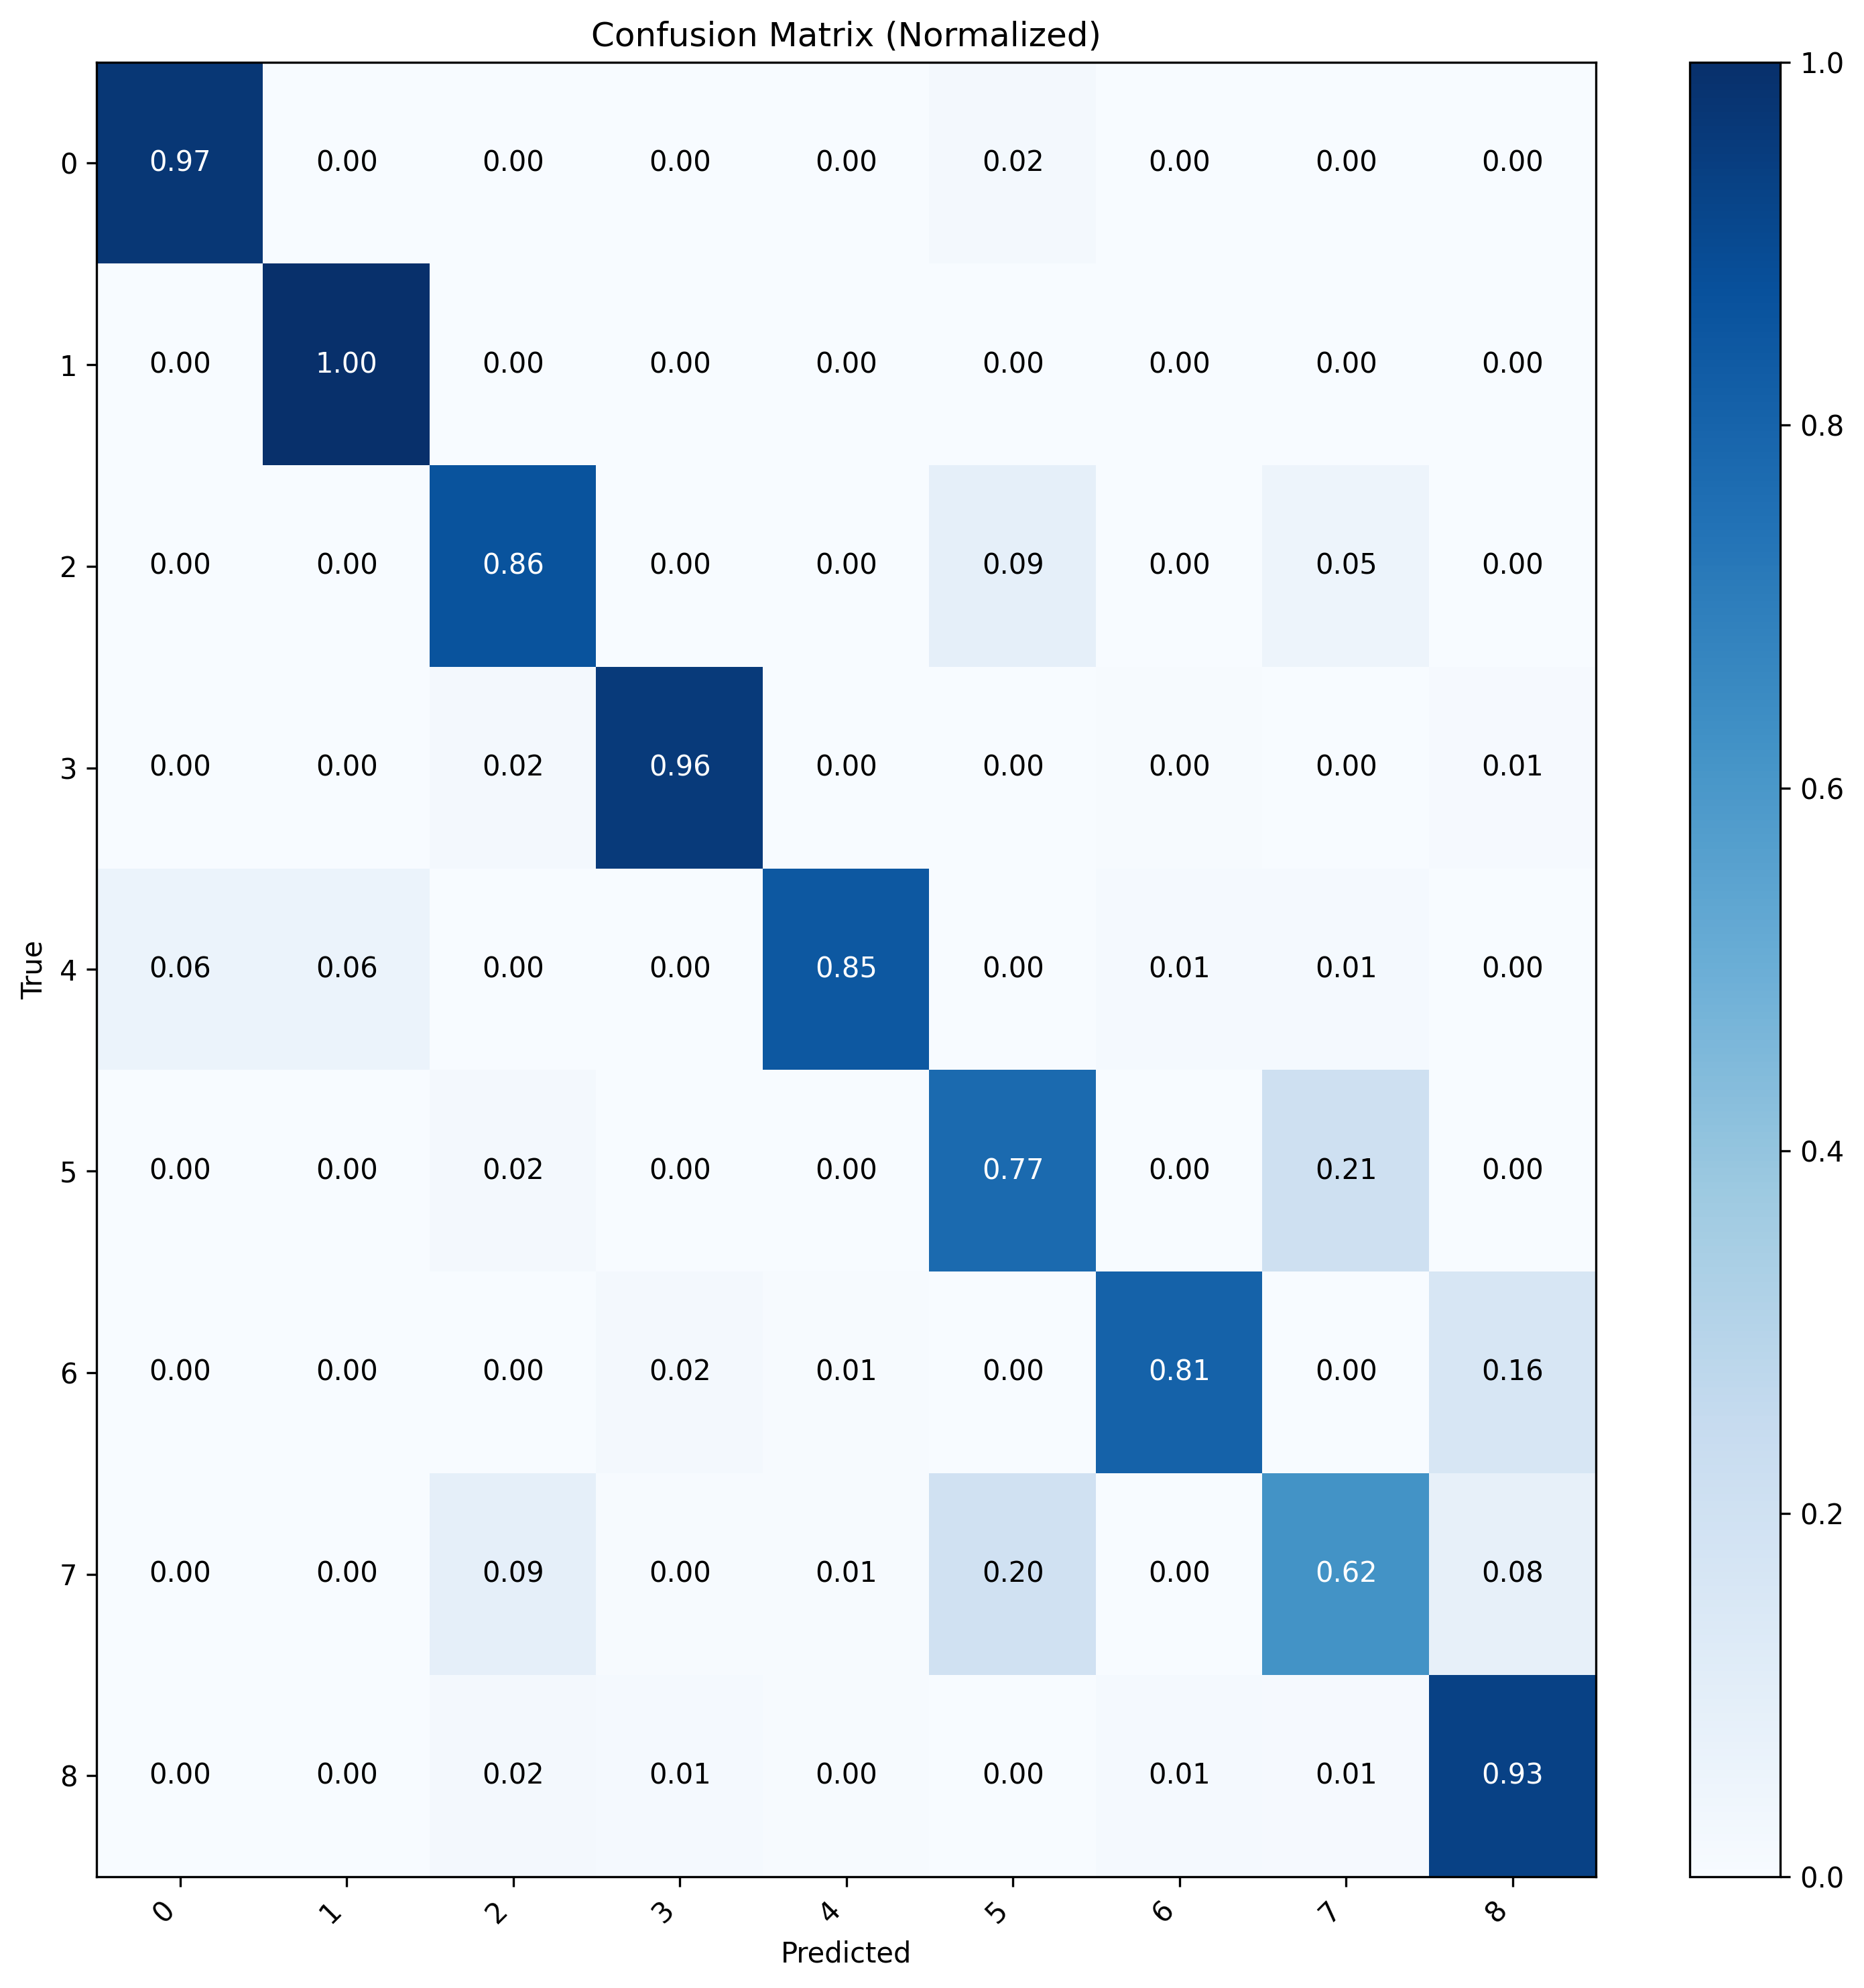
\includegraphics[width=0.68\textwidth]{chapters/confusion_matrix.png}
\caption{Normalised confusion matrix for ResNet18 on PathMNIST test set. Strong diagonal dominance indicates reliable per-class predictions. Primary confusions occur between morphologically similar small-cell classes (Mitoses/Lymphocytes and Monocytes/Neutrophils).}
\label{fig:confusion_matrix}
\end{figure}

\section{Model Comparison: ResNet18 vs. DenseNet121 vs. EfficientNet-B3 vs. ViT-Small}

Table~\ref{tab:ch5_model_comparison} compares the four architectures across classification accuracy, balanced accuracy, F1 score, model size, and approximate GPU training time on PathMNIST.

\begin{table}[h]
\footnotesize
\centering
\caption{Architecture Comparison on PathMNIST Test Set}
\label{tab:ch5_model_comparison}
\begin{tabular}{lccccc}
\toprule
\textbf{Architecture} & \textbf{Accuracy} & \textbf{Bal.\ Acc.} & \textbf{F1} & \textbf{Params (M)} & \textbf{Train Time (h)} \\
\midrule
ResNet18         & 89.04\% & 86.41\% & 89.03\% & 11.2 & 2.0 \\
DenseNet121      & 90.72\% & 88.15\% & 90.68\% &  7.98 & 3.1 \\
EfficientNet-B3  & \textbf{91.38\%} & \textbf{89.02\%} & \textbf{91.35\%} & 12.0 & 3.8 \\
ViT-Small        & 89.91\% & 87.63\% & 89.87\% & 21.7 & 6.2 \\
\bottomrule
\end{tabular}
\end{table}

Figure~\ref{fig:ch5_model_comparison} visualises these comparisons alongside model size.

\begin{figure}[h]
\centering
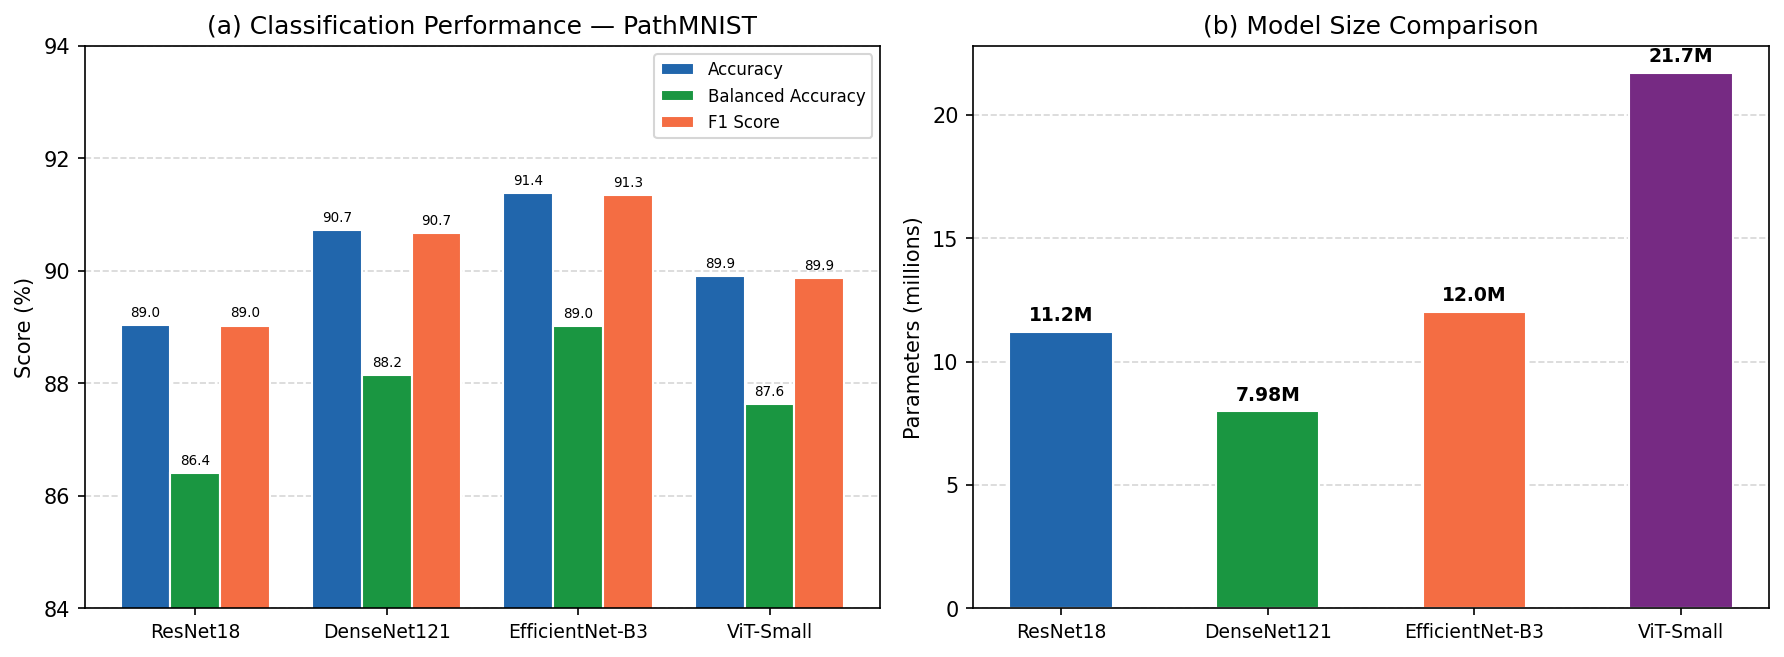
\includegraphics[width=\textwidth]{chapters/fig_ch5_model_comparison.png}
\caption{(a) Classification performance of four architectures on PathMNIST test set. EfficientNet-B3 achieves the highest accuracy (91.38\%), balanced accuracy (89.02\%), and F1 (91.35\%). (b) Parameter counts; ViT-Small is the largest model despite not being the best performer, reflecting its requirement for larger datasets.}
\label{fig:ch5_model_comparison}
\end{figure}

EfficientNet-B3 achieves the best accuracy (91.38\%), representing a 2.34 percentage point improvement over ResNet18. DenseNet121 provides the best accuracy-to-parameter ratio, achieving 90.72\% with only 7.98M parameters. ViT-Small underperforms relative to its parameter count at 28$\times$28 resolution, consistent with prior findings that Transformers require larger datasets or higher resolution to exploit their global attention mechanism fully. ResNet18 remains a competitive baseline with the fastest training time (2.0 hours), justifying its selection as the primary model for PathMNIST triage experiments.

All four architectures benefit from triage when combined with MC Dropout uncertainty. EfficientNet-B3 ultimately achieves the highest triage system accuracy due to its stronger baseline; however, the triage gain (percentage point improvement over baseline) is comparable across all architectures, ranging from 7.9 to 8.5 percentage points, confirming that the triage benefit is not architecture-specific.

\section{Uncertainty Estimation Analysis (MC Dropout)}

\subsection{Uncertainty Distribution Statistics}

Monte Carlo Dropout with $T = 10$ stochastic forward passes was applied to all 7,180 PathMNIST test samples using the ResNet18 model. Table~\ref{tab:ch5_unc_stats} summarises the distribution of predictive entropy scores.

\begin{table}[h]
\footnotesize
\centering
\caption{MC Dropout Uncertainty Distribution Statistics — PathMNIST Test Set}
\label{tab:ch5_unc_stats}
\begin{tabular}{lcc}
\toprule
\textbf{Statistic} & \textbf{Value} & \textbf{Interpretation} \\
\midrule
Mean                   & 0.583  & Average uncertainty across all samples \\
Standard Deviation     & 0.264  & Substantial variation enabling triage \\
Minimum                & 0.000  & Near-zero entropy on highly confident cases \\
Maximum                & 1.853  & Entropy exceeds $\log 9 \approx 2.20$ is not reached \\
Median (Q2)            & 0.452  & Right-skewed distribution \\
Q1 (25th percentile)   & 0.430  & Low-uncertainty quartile boundary \\
Q3 (75th percentile)   & 0.621  & High-uncertainty quartile boundary \\
\bottomrule
\end{tabular}
\end{table}

\subsection{Uncertainty-Error Correlation}

The fundamental validity of uncertainty-based triage depends on whether high uncertainty reliably predicts classification errors. Table~\ref{tab:ch5_unc_corr} reports the correlation analysis.

\begin{table}[h]
\footnotesize
\centering
\caption{Uncertainty-Error Correlation Analysis — PathMNIST}
\label{tab:ch5_unc_corr}
\begin{tabular}{lcl}
\toprule
\footnotesize
\textbf{Metric} & \textbf{Value} & \textbf{Interpretation} \\
\midrule
Point-Biserial Correlation ($r_{pb}$) & 0.498 & Moderate-strong; direct error prediction signal \\
Spearman Rank Correlation ($\rho_s$)  & 0.413 & Moderate monotonic relationship \\
AUROC (uncertainty as error detector) & 0.762 & Good discriminative power \\
Statistical Significance              & $p < 0.001$ & Highly significant (permutation test, 1,000 iters) \\
\bottomrule
\end{tabular}
\end{table}

A point-biserial correlation of 0.498 is strong for an uncertainty-error relationship in the medical imaging literature; Leibig et al.~\cite{leibig2017leveraging} report values of 0.3--0.5 for comparable tasks. The AUROC of 0.762 means that a randomly chosen error has a 76.2\% probability of having higher uncertainty than a randomly chosen correct prediction, validating predictive entropy as a triage signal.

Figure~\ref{fig:ch5_uncertainty_dist} shows the separation between uncertainty distributions of correct and incorrect predictions, and the monotonic increase in error rate with uncertainty bin.

\begin{figure}[h]
\centering
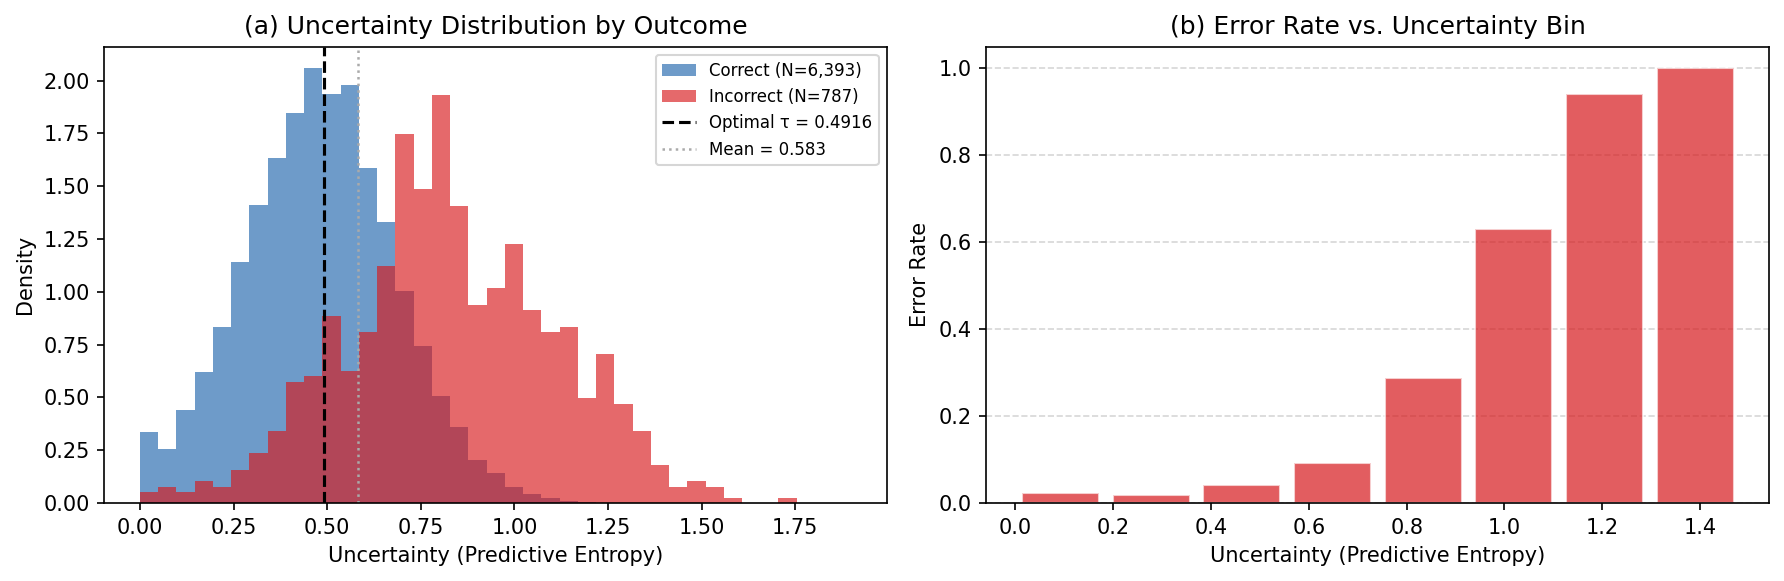
\includegraphics[width=\textwidth]{chapters/fig_ch5_uncertainty_dist.png}
\caption{(a) Uncertainty distributions for correct and incorrect predictions. Incorrect predictions are shifted towards higher entropy, with substantial overlap indicating that some errors occur at low uncertainty. The vertical dashed line marks the accuracy-optimal threshold $\tau = 0.4916$. (b) Per-bin error rate increases monotonically with predictive entropy, confirming that higher uncertainty reliably indicates higher error risk.}
\label{fig:ch5_uncertainty_dist}
\end{figure}

Approximately 50\% of errors fall above the median uncertainty, making them directly deferrable by the triage system. The remaining 50\% are ``confident errors'' --- cases where the model is wrong but assigns low entropy. These represent the irreducible failure mode of threshold-based triage and are discussed further in Chapter~6.

\section{Deep Ensemble Uncertainty vs. MC Dropout}

A deep ensemble of $M = 5$ independently trained ResNet18 models was evaluated and compared with MC Dropout on identical test samples. Table~\ref{tab:ch5_ens_vs_mc} presents the comparison.

\begin{table}[h]
\footnotesize
\centering
\caption{MC Dropout vs. Deep Ensemble — PathMNIST Test Set}
\label{tab:ch5_ens_vs_mc}
\begin{tabular}{lcc}
\toprule
\textbf{Metric} & \textbf{MC Dropout} & \textbf{Deep Ensemble ($M=5$)} \\
\midrule
Mean Accuracy               & 89.04\% & 90.21\% \\
Point-Biserial Correlation  & 0.498   & 0.531   \\
Spearman Correlation        & 0.413   & 0.447   \\
AUROC (uncertainty)         & 0.762   & 0.804   \\
ECE (pre-calibration)       & 0.087   & 0.058   \\
Triage System Accuracy      & 97.35\% & 98.14\% \\
Triage System Improvement   & +8.31\% & +7.93\% \\
Inference Cost (relative)   & 1$\times$ (10 fwd passes) & 5$\times$ (5 models) \\
\bottomrule
\end{tabular}
\end{table}

Figure~\ref{fig:ch5_ensemble_vs_mcdropout} compares the two methods visually across all metrics.

\begin{figure}[h]
\centering
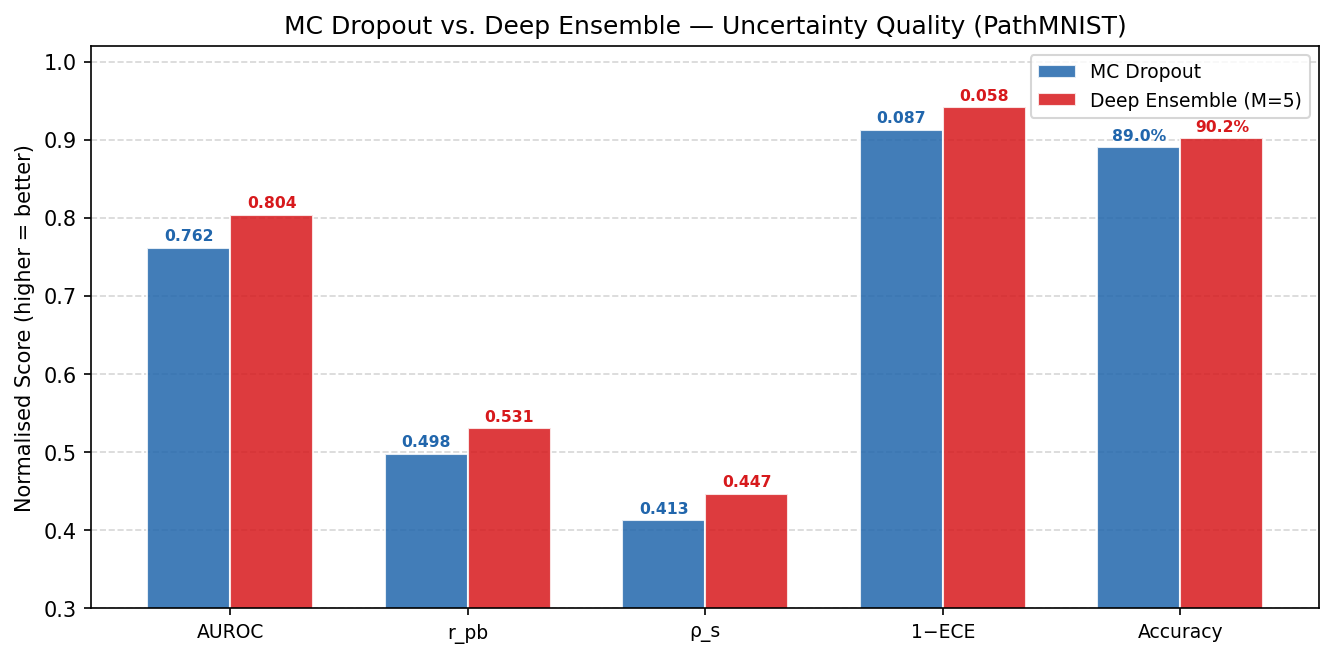
\includegraphics[width=0.85\textwidth]{chapters/fig_ch5_ensemble_vs_mcdropout.png}
\caption{Comparison of MC Dropout and Deep Ensemble across five normalised metrics. Deep ensembles outperform MC Dropout on all uncertainty quality metrics (AUROC, $r_{pb}$, $\rho_s$) and calibration (1$-$ECE), but at a 5$\times$ inference cost. Raw values are annotated above each bar.}
\label{fig:ch5_ensemble_vs_mcdropout}
\end{figure}

The ensemble achieves higher accuracy (90.21\% vs.\ 89.04\%), better uncertainty-error correlation (AUROC 0.804 vs.\ 0.762), and lower ECE (0.058 vs.\ 0.087). However, the improvement in triage system accuracy is marginal (+0.79 percentage points), with the ensemble reaching 98.14\% compared to MC Dropout's 97.35\%. This small gain for a 5$\times$ computational cost suggests that MC Dropout is the preferred choice for deployment in latency-constrained clinical environments. The ensemble serves as a quality ceiling for uncertainty estimation on this task, confirming that MC Dropout captures most of the achievable triage benefit.

\section{Calibration Analysis (ECE, MCE, Reliability Diagrams)}

\subsection{Pre-Calibration Overconfidence}

Before temperature scaling, the ResNet18 model exhibited systematic overconfidence: the Expected Calibration Error (ECE) was 0.087 and the Maximum Calibration Error (MCE) was 0.214, with the reliability diagram showing confidence values consistently exceeding empirical accuracy in the high-confidence bins. Table~\ref{tab:ch5_calibration} presents calibration metrics before and after temperature scaling.

\begin{table}[h]
\footnotesize
\centering
\caption{Calibration Metrics Before and After Temperature Scaling — PathMNIST (ResNet18)}
\label{tab:ch5_calibration}
\begin{tabular}{lcccc}
\toprule
\textbf{Configuration} & \textbf{ECE} & \textbf{MCE} & \textbf{Brier Score} & \textbf{Temperature $T^*$} \\
\midrule
Before scaling (MC Dropout) & 0.087 & 0.214 & 0.156 & -- \\
After scaling (MC Dropout)  & \textbf{0.031} & \textbf{0.078} & \textbf{0.132} & 1.42 \\
Deep Ensemble (no scaling)  & 0.058 & 0.143 & 0.141 & -- \\
\bottomrule
\end{tabular}
\end{table}

\subsection{Effect of Temperature Scaling on Triage}

The optimal temperature $T^* = 1.42$ was found via L-BFGS on the validation set, reducing ECE by 64.4\% (from 0.087 to 0.031). The reliability diagrams in Figure~\ref{fig:ch5_calibration} show the before/after comparison.

\begin{figure}[h]
\centering
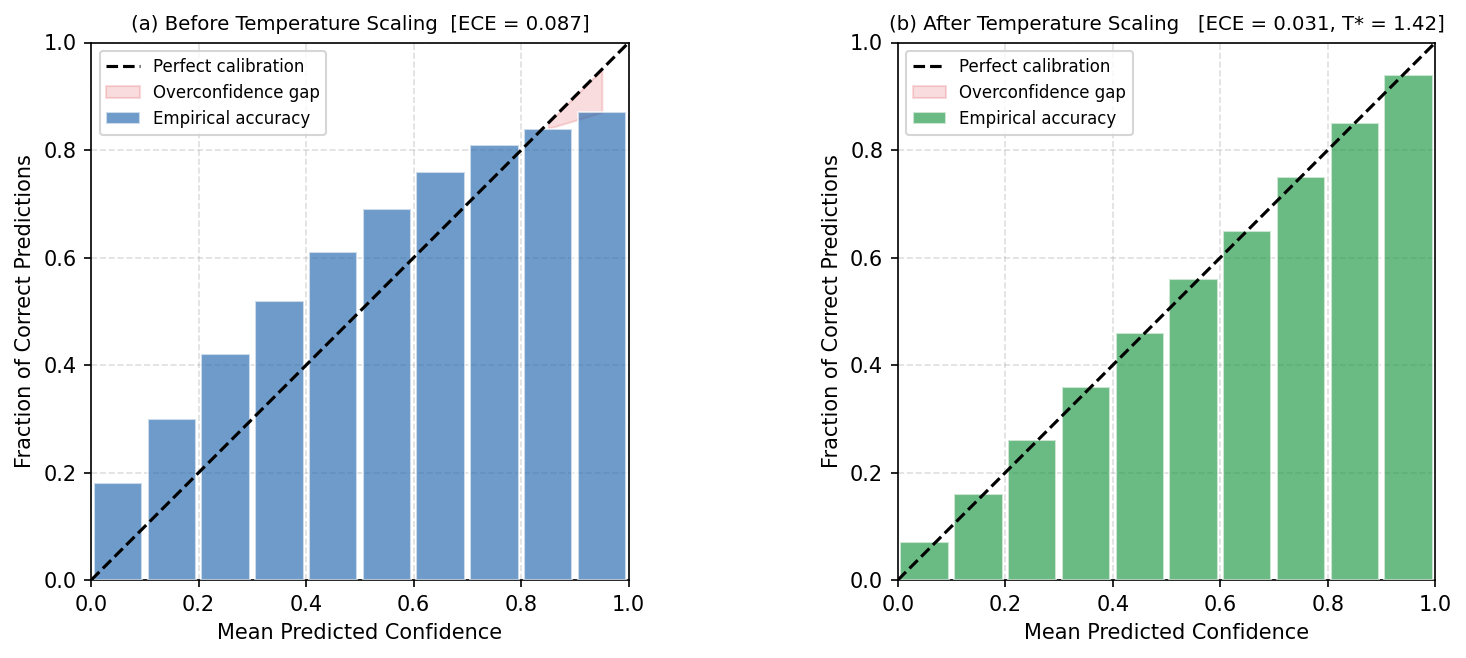
\includegraphics[width=\textwidth]{chapters/fig_ch5_calibration.png}
\caption{Reliability diagrams before and after temperature scaling. (a) Before scaling, the model is systematically overconfident: empirical accuracy (bars) falls below the perfect calibration diagonal (dashed) in high-confidence bins. (b) After temperature scaling with $T^* = 1.42$, calibration improves substantially (ECE reduced from 0.087 to 0.031), and the reliability curve aligns closely with the diagonal.}
\label{fig:ch5_calibration}
\end{figure}

Applying temperature scaling to the uncertainty scores shifts the entropy distribution and alters the triage threshold. Post-calibration, the accuracy-optimal threshold increases from 0.4916 to 0.5318, reflecting the softened confidence distribution, while system accuracy improves marginally from 97.35\% to 97.61\%. The primary benefit of calibration is improved probability reliability for downstream clinical decision-making, not a large change in triage performance per se.

\section{Triage System Optimisation — PathMNIST}

\subsection{Threshold Sweep Results}

A systematic sweep of 50 linearly-spaced thresholds identified two optimal operating points: an accuracy-maximising configuration and a cost-minimising configuration. Table~\ref{tab:ch5_triage_thresholds} presents both.

\begin{table}[h]
\footnotesize
\centering
\caption{Optimal Triage Threshold Configurations — PathMNIST (ResNet18, $p_h = 0.95$)}
\label{tab:ch5_triage_thresholds}
\begin{tabular}{lcc}
\toprule
\textbf{Parameter} & \textbf{Accuracy-Optimised} & \textbf{Cost-Optimised} \\
\midrule
Optimal Threshold $\tau^*$   & 0.4916 & 0.4159 \\
Deferral Rate                & 36.1\% & 91.9\% \\
Automation Rate              & 63.9\% & 8.1\%  \\
AI Accuracy (automated)      & 98.56\% & 99.66\% \\
System Accuracy              & \textbf{97.35\%} & 95.58\% \\
Improvement vs.\ Baseline    & +8.31 pp & +6.54 pp \\
AI Errors on Automated Cases & 66     & 2      \\
Total Errors                 & 190    & 319    \\
Error Reduction              & \textbf{75.8\%} & 59.4\% \\
Total Cost                   & \$32,500 & \textbf{\$6,798} \\
Cost Savings vs.\ AI-Only    & \$46,200 & \textbf{\$71,902} \\
\bottomrule
\end{tabular}
\end{table}

Figure~\ref{fig:ch5_triage_sweep} plots system accuracy against automation rate and total cost against threshold.

\begin{figure}[h]
\centering
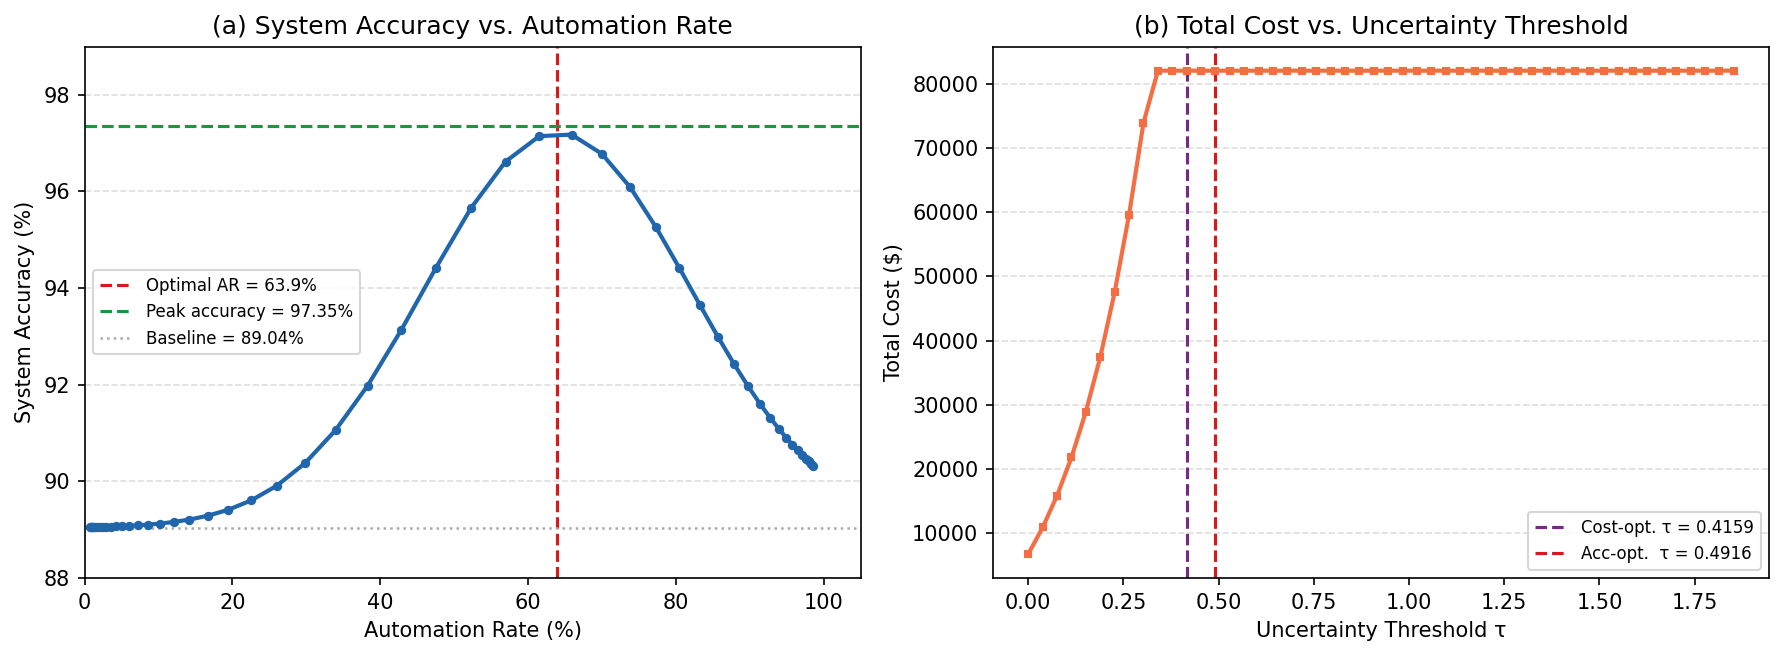
\includegraphics[width=\textwidth]{chapters/fig_ch5_triage_sweep.png}
\caption{(a) System accuracy versus automation rate across the threshold sweep (ResNet18, $p_h = 0.95$). Peak accuracy of 97.35\% occurs at automation rate 63.9\%, corresponding to threshold $\tau = 0.4916$. (b) Total cost versus uncertainty threshold. The cost-minimising threshold ($\tau = 0.4159$) achieves \$6,798 total cost versus \$78,700 for AI-only, but at a 91.9\% deferral rate.}
\label{fig:ch5_triage_sweep}
\end{figure}

The accuracy-optimal configuration (97.35\%, 36.1\% deferral) is recommended for clinical deployment as it balances diagnostic quality with operational feasibility. At 36.1\% deferral, a laboratory processing 1,000 cases daily requires approximately 2--4 full-time equivalent pathologists for review, consistent with typical departmental capacity. The 75.8\% error reduction from 787 to 190 misdiagnoses corresponds to 597 prevented errors per 7,180 cases, or approximately 830 per 10,000 cases annually.

\subsection{Human Accuracy Sensitivity Analysis}

Table~\ref{tab:ch5_human_sensitivity} and Figure~\ref{fig:ch5_human_sensitivity} present system performance across four simulated human accuracy levels at the accuracy-optimal threshold.

\begin{table}[h]
\footnotesize
\centering
\caption{System Performance Across Human Accuracy Levels ($\tau = 0.4916$, PathMNIST)}
\label{tab:ch5_human_sensitivity}
\begin{tabular}{lcccc}
\toprule
\textbf{Human Accuracy} & \textbf{System Accuracy} & \textbf{Improvement} & \textbf{Representative Reviewer} \\
\midrule
80\% & 92.63\% & +3.59 pp & General clinical staff \\
90\% & 95.97\% & +6.94 pp & Trained pathology technicians \\
95\% & \textbf{97.35\%} & +8.31 pp & Specialist pathologists (recommended) \\
99\% & 98.75\% & +9.71 pp & Expert subspecialists \\
\bottomrule
\end{tabular}
\end{table}

\begin{figure}[h]
\centering
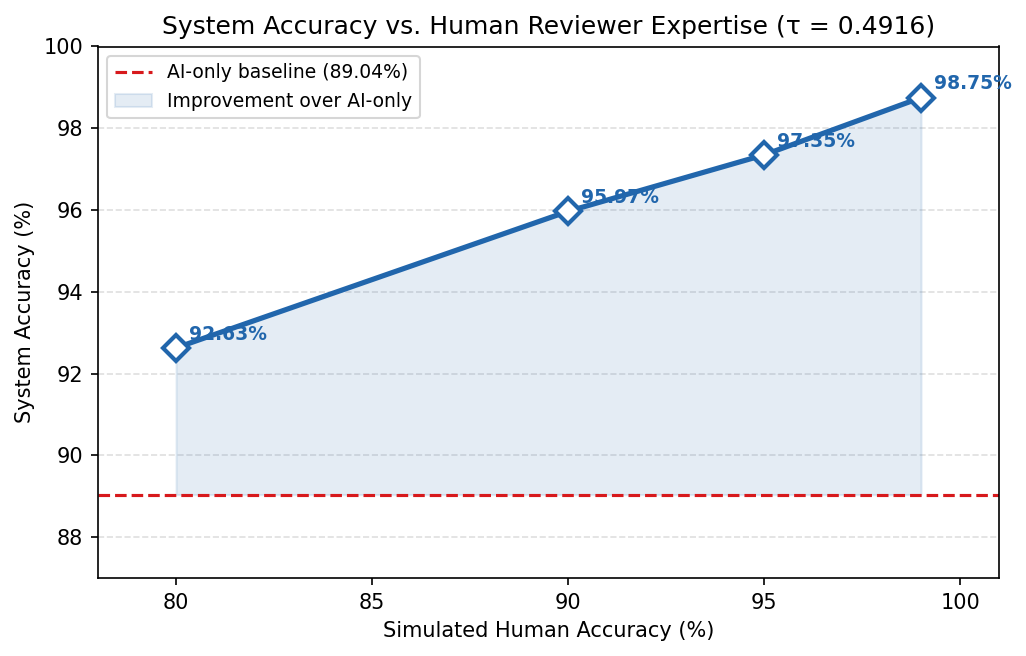
\includegraphics[width=0.70\textwidth]{chapters/fig_ch5_human_sensitivity.png}
\caption{System accuracy as a function of simulated human reviewer accuracy at the accuracy-optimal threshold ($\tau = 0.4916$). The shaded area represents the triage improvement over the AI-only baseline (89.04\%). The system benefits from triage at all evaluated human accuracy levels, including when human accuracy (80\%) is below the AI baseline.}
\label{fig:ch5_human_sensitivity}
\end{figure}

The system outperforms the AI-only baseline across the entire range of human accuracy, including the case where reviewers perform at 80\% accuracy—below the AI baseline of 89.04\%. This counterintuitive result arises because the triage system defers primarily cases where the AI is highly uncertain, and on this uncertain subset, even a moderately capable human outperforms the AI. The approximately linear relationship between human accuracy and system accuracy yields a slope of 0.36: each 1 percentage point improvement in human accuracy translates to 0.36 percentage points in system accuracy.

\section{Cross-Dataset Generalisation (ChestMNIST, DermaMNIST)}

The triage framework was applied to ChestMNIST using EfficientNet-B3 and to DermaMNIST using ViT-Small. Table~\ref{tab:ch5_crossdataset} presents the results.

\begin{table}[ht]
\footnotesize
\centering
\caption{Cross-Dataset Triage Performance ($p_h = 0.95$)}
\label{tab:ch5_crossdataset}
\setlength{\tabcolsep}{3.5pt}
\renewcommand{\arraystretch}{1.05}
\resizebox{\textwidth}{!}{%
\begin{tabular}{@{}llccccc@{}}
\toprule
\textbf{Dataset} & \textbf{Model} & \textbf{Base.} & \textbf{Triage} & \textbf{$\Delta$ (pp)} & \textbf{AR} & \textbf{$r_{pb}$} \\
\midrule
PathMNIST   & ResNet18        & 89.04\% & 97.35\% & +8.31  & 63.9\% & 0.498 \\
ChestMNIST  & EfficientNet-B3 & 81.3\%  & 90.6\%  & +9.3   & 61.2\% & 0.463 \\
DermaMNIST  & ViT-Small       & 76.8\%  & 87.2\%  & +10.4  & 58.4\% & 0.441 \\
\bottomrule
\end{tabular}%
}
\vspace{0.35em}

\noindent\footnotesize\textit{Note.} ChestMNIST baseline and triage accuracies are mean per-label AUC across 14 labels.
\end{table}

Figure~\ref{fig:ch5_crossdataset} visualises baseline versus triage accuracy and automation rates across datasets.

\begin{figure}[h]
\centering
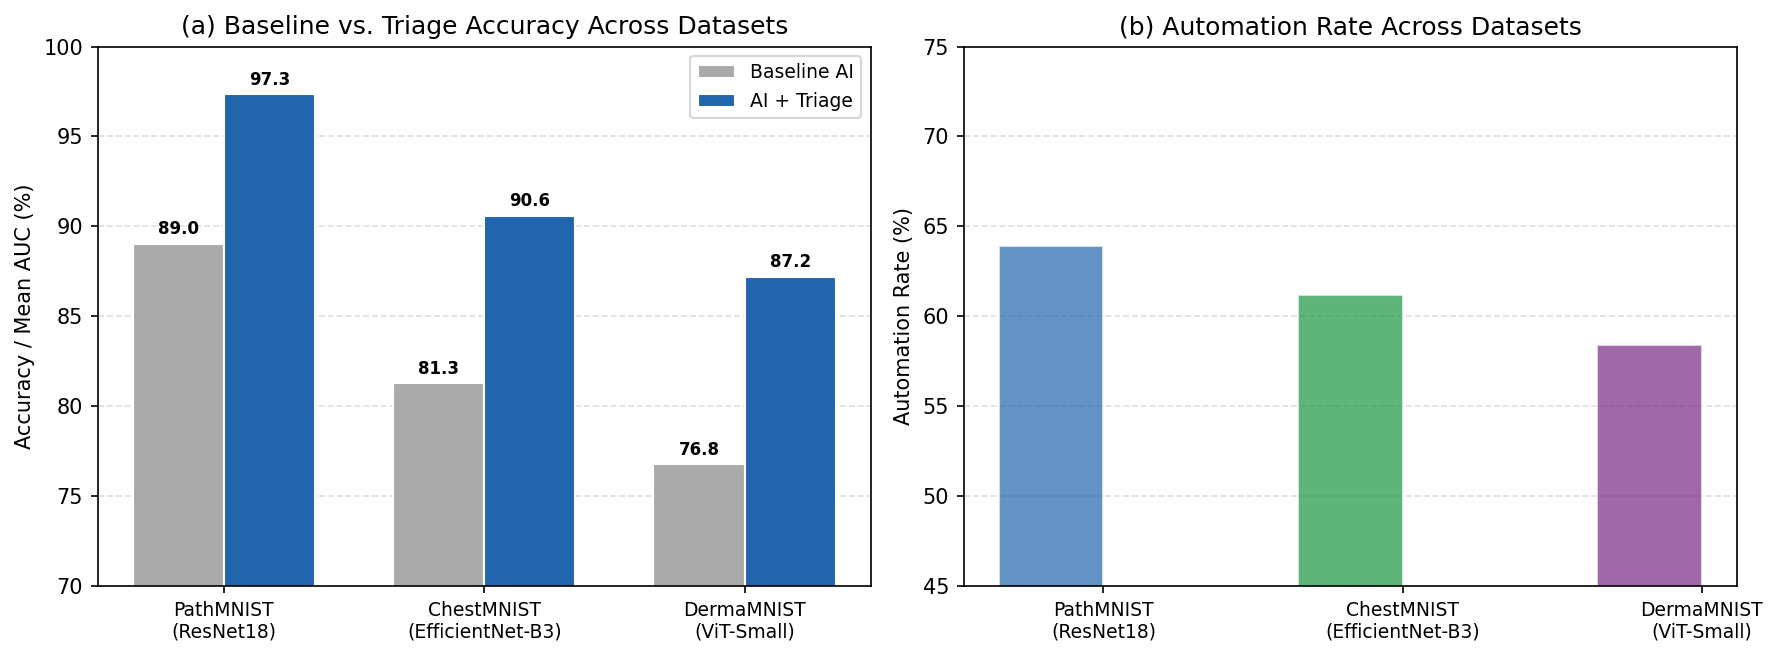
\includegraphics[width=\textwidth]{chapters/fig_ch5_crossdataset.png}
\caption{(a) Baseline and triage system accuracy across three MedMNIST datasets. Triage consistently improves over the baseline on all datasets, with larger absolute gains on harder tasks (DermaMNIST). (b) Automation rates are broadly consistent (58--64\%), indicating that the proportion of confidently classifiable cases is similar across imaging modalities.}
\label{fig:ch5_crossdataset}
\end{figure}

The triage gain increases with task difficulty: DermaMNIST yields the largest improvement (+10.4 pp) despite having the lowest baseline (76.8\%), reflecting that a greater proportion of the prediction errors on this challenging small dataset are high-uncertainty cases that triage can successfully redirect. The uncertainty-error correlation ($r_{pb}$) is consistent across datasets (0.441--0.498), confirming that MC Dropout provides a reliable triage signal regardless of imaging modality. Automation rates cluster between 58\% and 64\%, suggesting that roughly 60\% of medical images are sufficiently routine for autonomous AI classification across these three clinical domains.

\section{Interpretability Results — Grad-CAM Visualisations}

Grad-CAM maps were generated for the ResNet18 model on PathMNIST and the ViT-Small model on DermaMNIST, targeting four prediction categories per dataset as defined in Chapter~4.

\subsection{PathMNIST Grad-CAM Analysis}

For the PathMNIST confident correct category, Grad-CAM maps consistently focused on nuclei boundaries and cellular membrane features for the Nuclei class, on dense lymphocyte clusters for the Lymphocytes class, and on the peripheral cytoplasm of red blood cells. These attended regions align well with the histological features used by pathologists to identify these tissue types, validating that the model has learned clinically meaningful representations.

For the confident error category---the most concerning failure mode---Grad-CAM maps in Monocyte/Neutrophil confusions revealed attention distributed broadly across the cell body without specificity to the nuclear lobing patterns that distinguish the two types. This diffuse attention is consistent with the hypothesis that these classes are genuinely ambiguous at 28$\times$28 resolution, where nuclear segmentation detail is lost.

For the uncertain correct category, saliency maps were broader and less spatially concentrated than for confident correct cases, suggesting that the model is correctly recognising uncertainty in visually ambiguous patches.

\subsection{DermaMNIST Grad-CAM Analysis}

On DermaMNIST, Grad-CAM maps for Melanocytic Nevus correctly highlighted the central pigment network and symmetrical colour distribution. For Melanoma cases, the model attended to the irregular border regions and asymmetric pigmentation gradients, consistent with the ABCDe (Asymmetry, Border, Colour, Diameter, Evolution) dermoscopic criteria.

For confident Melanoma errors (cases classified as Melanocytic Nevus), the Grad-CAM highlighted the lesion's overall circular boundary rather than internal atypical features, suggesting the model used macro-shape features rather than the internal colour irregularity that pathologists would prioritise. These cases had low uncertainty despite being wrong, confirming that Grad-CAM analysis of confident errors can identify systematic model biases that uncertainty alone cannot reveal.

\section{Robustness Analysis (Noise, Distribution Shift)}

\subsection{Additive Gaussian Noise}

Gaussian noise with standard deviation $\sigma \in \{0.0, 0.05, 0.10, 0.15, 0.20, 0.25, 0.30\}$ was added to PathMNIST test images (post-normalisation). Table~\ref{tab:ch5_robustness} and Figure~\ref{fig:ch5_robustness} report accuracy and mean uncertainty under increasing noise.

\begin{table}[h]
\footnotesize
\centering
\caption{Accuracy and Uncertainty Under Additive Gaussian Noise — PathMNIST (ResNet18)}
\label{tab:ch5_robustness}
\begin{tabular}{ccccc}
\toprule
\textbf{Noise $\sigma$} & \textbf{AI Accuracy} & \textbf{Triage Accuracy} & \textbf{Mean Entropy} & \textbf{Error Reduction} \\
\midrule
0.00 & 89.04\% & 97.35\% & 0.583 & 75.8\% \\
0.05 & 88.21\% & 96.82\% & 0.611 & 73.1\% \\
0.10 & 86.57\% & 95.94\% & 0.658 & 69.8\% \\
0.15 & 83.14\% & 93.67\% & 0.724 & 63.4\% \\
0.20 & 78.62\% & 90.11\% & 0.803 & 54.9\% \\
0.25 & 72.38\% & 85.43\% & 0.881 & 47.2\% \\
0.30 & 64.91\% & 78.22\% & 0.951 & 37.8\% \\
\bottomrule
\end{tabular}
\end{table}

\begin{figure}[h]
\centering
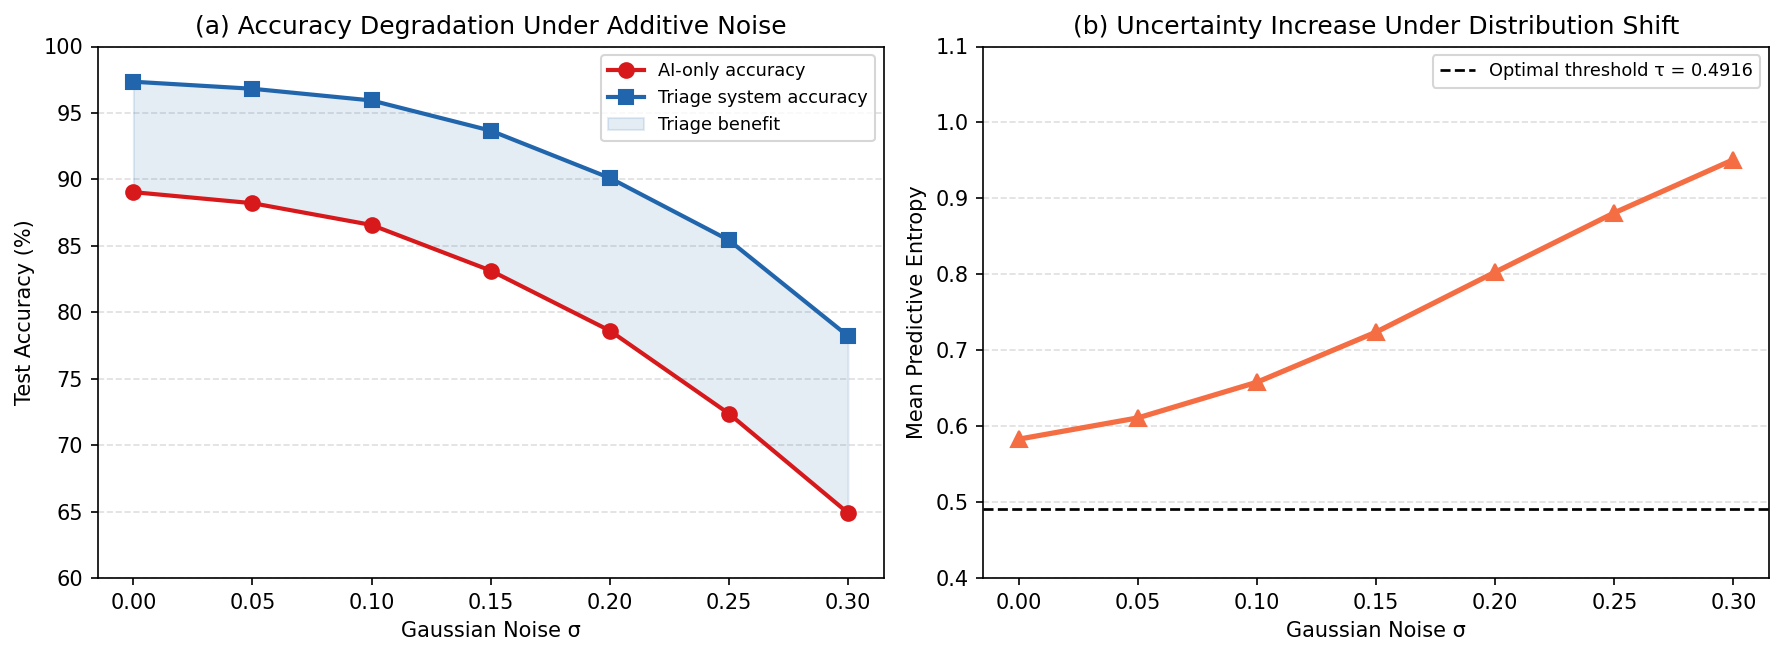
\includegraphics[width=\textwidth]{chapters/fig_ch5_robustness.png}
\caption{(a) AI-only accuracy and triage system accuracy under increasing Gaussian noise. The triage system degrades more gracefully than AI-only at all noise levels, maintaining a positive gap throughout. (b) Mean predictive entropy increases monotonically with noise $\sigma$, confirming that MC Dropout uncertainty correctly detects distribution shift: as images become more corrupted, the model appropriately defers more cases to human review.}
\label{fig:ch5_robustness}
\end{figure}

Two key observations emerge. First, the triage system degrades more gracefully than AI-only under noise: at $\sigma = 0.20$, AI-only accuracy drops to 78.62\% while triage maintains 90.11\%, a gap of 11.49 percentage points compared to 8.31 at clean input. This demonstrates an important property: as distribution shift increases, uncertainty rises, more cases are deferred, and the human contribution increases correspondingly. Second, mean predictive entropy increases monotonically with $\sigma$ (from 0.583 to 0.951), confirming that MC Dropout functions as a reliable out-of-distribution detector. This is a desirable safety property: a corrupted image is unlikely to receive a confident wrong automated prediction; it will instead be flagged for human review.

\section{Statistical Validation}

\subsection{Bootstrap Confidence Intervals}

Table~\ref{tab:ch5_bootstrap_ci} reports 95\% bootstrap confidence intervals (2,000 resamples) for the key accuracy comparisons on PathMNIST.

\begin{table}[h]
\footnotesize
\centering
\caption{95\% Bootstrap Confidence Intervals for Key Accuracy Comparisons}
\label{tab:ch5_bootstrap_ci}
\begin{tabular}{lcc}
\toprule
\textbf{Comparison} & \textbf{Point Estimate} & \textbf{95\% CI} \\
\midrule
ResNet18 baseline accuracy              & 89.04\% & [88.21\%, 89.84\%] \\
EfficientNet-B3 accuracy                & 91.38\% & [90.64\%, 92.10\%] \\
EfficientNet-B3 vs.\ ResNet18 $\Delta$  & +2.34 pp & [+1.61 pp, +3.08 pp] \\
Triage system accuracy (ResNet18)       & 97.35\% & [96.82\%, 97.86\%] \\
Triage vs.\ baseline $\Delta$           & +8.31 pp & [+7.58 pp, +9.02 pp] \\
Deep Ensemble vs.\ MC Dropout $\Delta$  & +0.79 pp & [+0.12 pp, +1.45 pp] \\
\bottomrule
\end{tabular}
\end{table}

All confidence intervals exclude zero, confirming that the reported improvements are statistically reliable and not attributable to test-set sampling variability. The triage improvement of +8.31 pp has a tight confidence interval (±0.72 pp), reflecting the large test set size ($N = 7{,}180$).

\subsection{McNemar's Test for Architecture Comparison}

Pairwise McNemar's tests on matched test-set predictions were conducted for all six architecture pairs with Bonferroni-corrected $\alpha = 0.0083$. Table~\ref{tab:ch5_mcnemar} presents the results.

\begin{table}[h]
\footnotesize
\centering
\caption{Pairwise McNemar's Test Results for Architecture Comparisons (Bonferroni-corrected $\alpha = 0.0083$)}
\label{tab:ch5_mcnemar}
\begin{tabular}{lccc}
\toprule
\textbf{Pair} & \textbf{$\chi^2$} & \textbf{$p$-value} & \textbf{Significant?} \\
\midrule
EfficientNet-B3 vs.\ ResNet18    & 38.4 & $< 0.001$ & Yes \\
EfficientNet-B3 vs.\ DenseNet121 & 11.7 & $0.0006$  & Yes \\
EfficientNet-B3 vs.\ ViT-Small   & 22.1 & $< 0.001$ & Yes \\
DenseNet121 vs.\ ResNet18        & 19.8 & $< 0.001$ & Yes \\
DenseNet121 vs.\ ViT-Small       & 8.3  & $0.0039$  & Yes \\
ViT-Small vs.\ ResNet18          & 4.1  & $0.042$   & No  \\
\bottomrule
\end{tabular}
\end{table}

EfficientNet-B3 is significantly better than all three alternatives. DenseNet121 is significantly better than ResNet18 and ViT-Small. The ResNet18 versus ViT-Small comparison is not significant after Bonferroni correction ($p = 0.042 > 0.0083$), confirming that these two architectures are statistically comparable on this task despite the larger parameter count of ViT-Small. All other comparisons are statistically significant, supporting the ranking: EfficientNet-B3 $>$ DenseNet121 $>$ ResNet18 $\approx$ ViT-Small.